%% V1.0
%% by Christopher Leith, udacl@cielsystems.com
%% This is a template for Udacity projects using IEEEtran.cls

\documentclass[10pt,journal,compsoc]{IEEEtran}

\usepackage[pdftex]{graphicx}    
\usepackage{cite}
\hyphenation{op-tical net-works semi-conduc-tor}

\begin{document}

\title{Deep RL Learning - Deep Reinforcement learning for robots}

\author{Christopher Leith}

\markboth{MapMyWorld, SLAM, Udacity}%
{}
\IEEEtitleabstractindextext{%

\begin{abstract}
In this project we create 
\end{abstract}

% Note that keywords are not normally used for peerreview papers.
\begin{IEEEkeywords}
Reinforement learning, Deep Learning, Robotics, ROS.
\end{IEEEkeywords}}


\maketitle
\IEEEdisplaynontitleabstractindextext
\IEEEpeerreviewmaketitle
\label{sec:Introduction}
\section{Introduction}
\IEEEPARstart{M}{obile} robots 
\section{Background / Formulation}
Because 

\subsection{RTABMap Slam}
In this project we demonstrate 
\begin{itemize}
 \item Wheel Odometry
 Measures the distance traveled be each wheel.
 \item Hokuyo Laser Rangefinder
 Mounted on top of the cylinder.
 \item RGB-Depth Camera
 Mounted on the front of the cylinder.
\end{itemize}



\section{Configuration}
Much Fig ~\ref{fig:rosgraph}.

\begin{figure}[h]
      \centering
      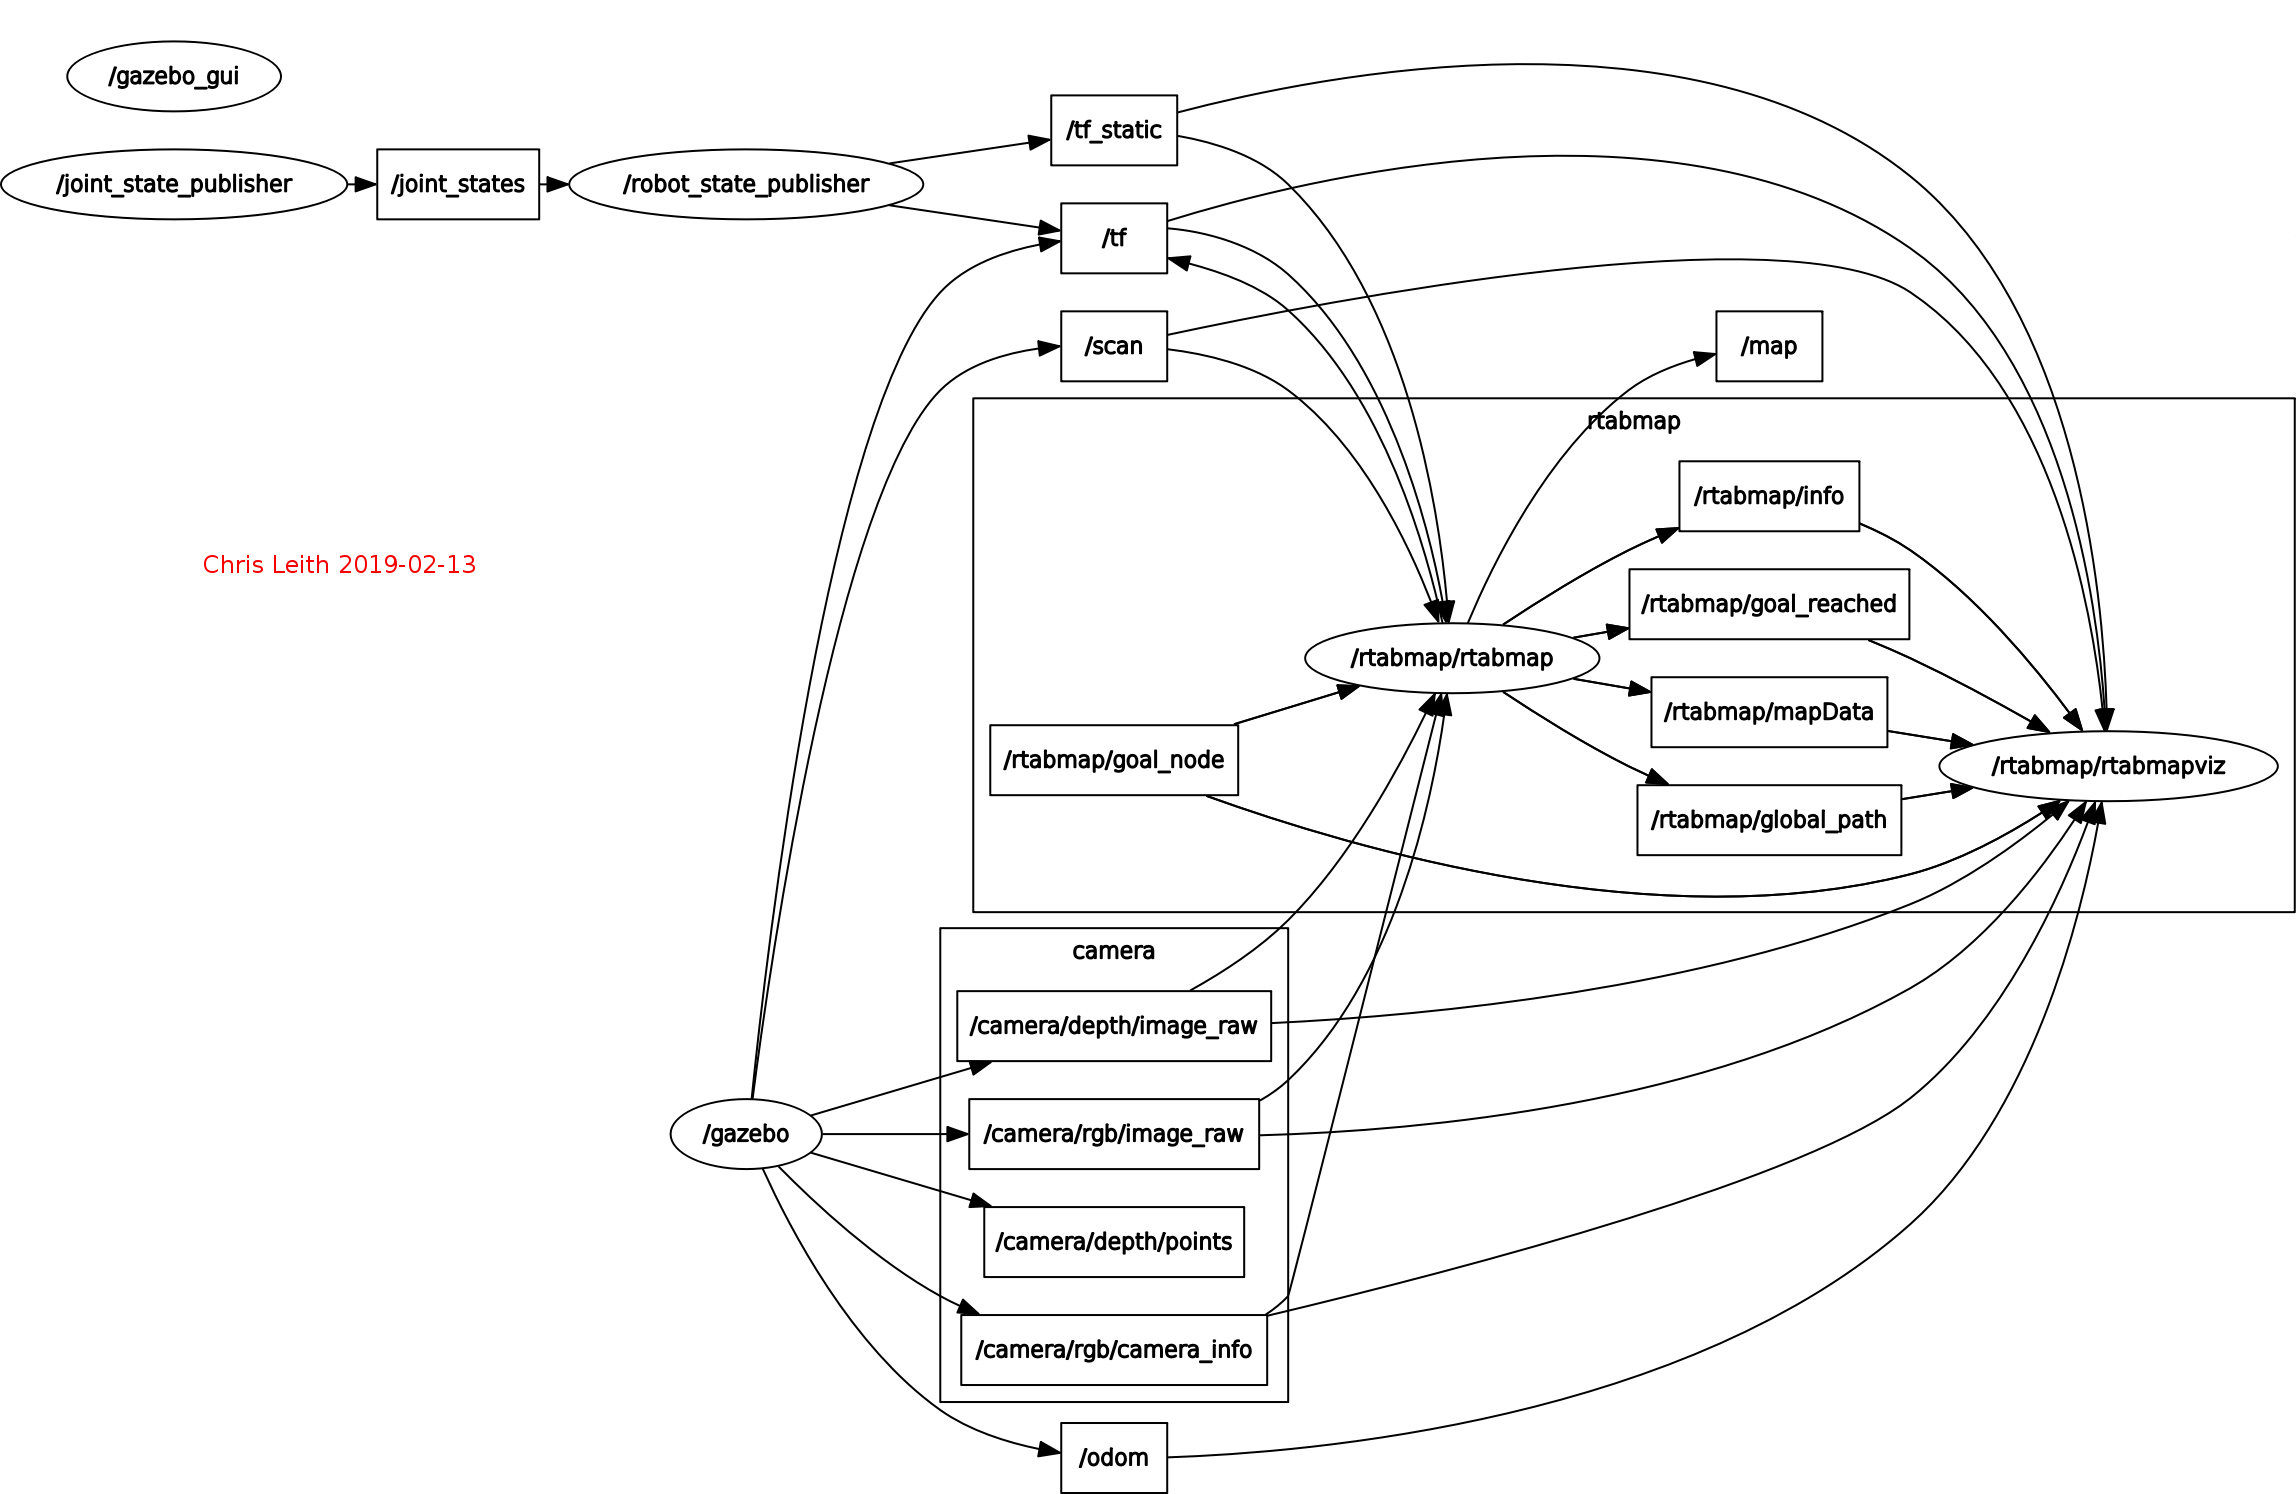
\includegraphics[width=\linewidth]{Assets/rosgraph_working.png}
      \caption{CielBot nodes and topics ROS Graph}
      \label{fig:rosgraph}
\end{figure}

\subsection{RTABMap Config}
 The configuration 
 
\subsection{Robot Config}
The robot used in this project,

\section{Results}
Map generation was reasonable, but not perfect as detailed below.
\subsection{Results - Kitchen and Dining World}
From Run1 Fig ~\ref{fig:kitchen_dbview_run1} 

\begin{figure}[h]
      \centering
      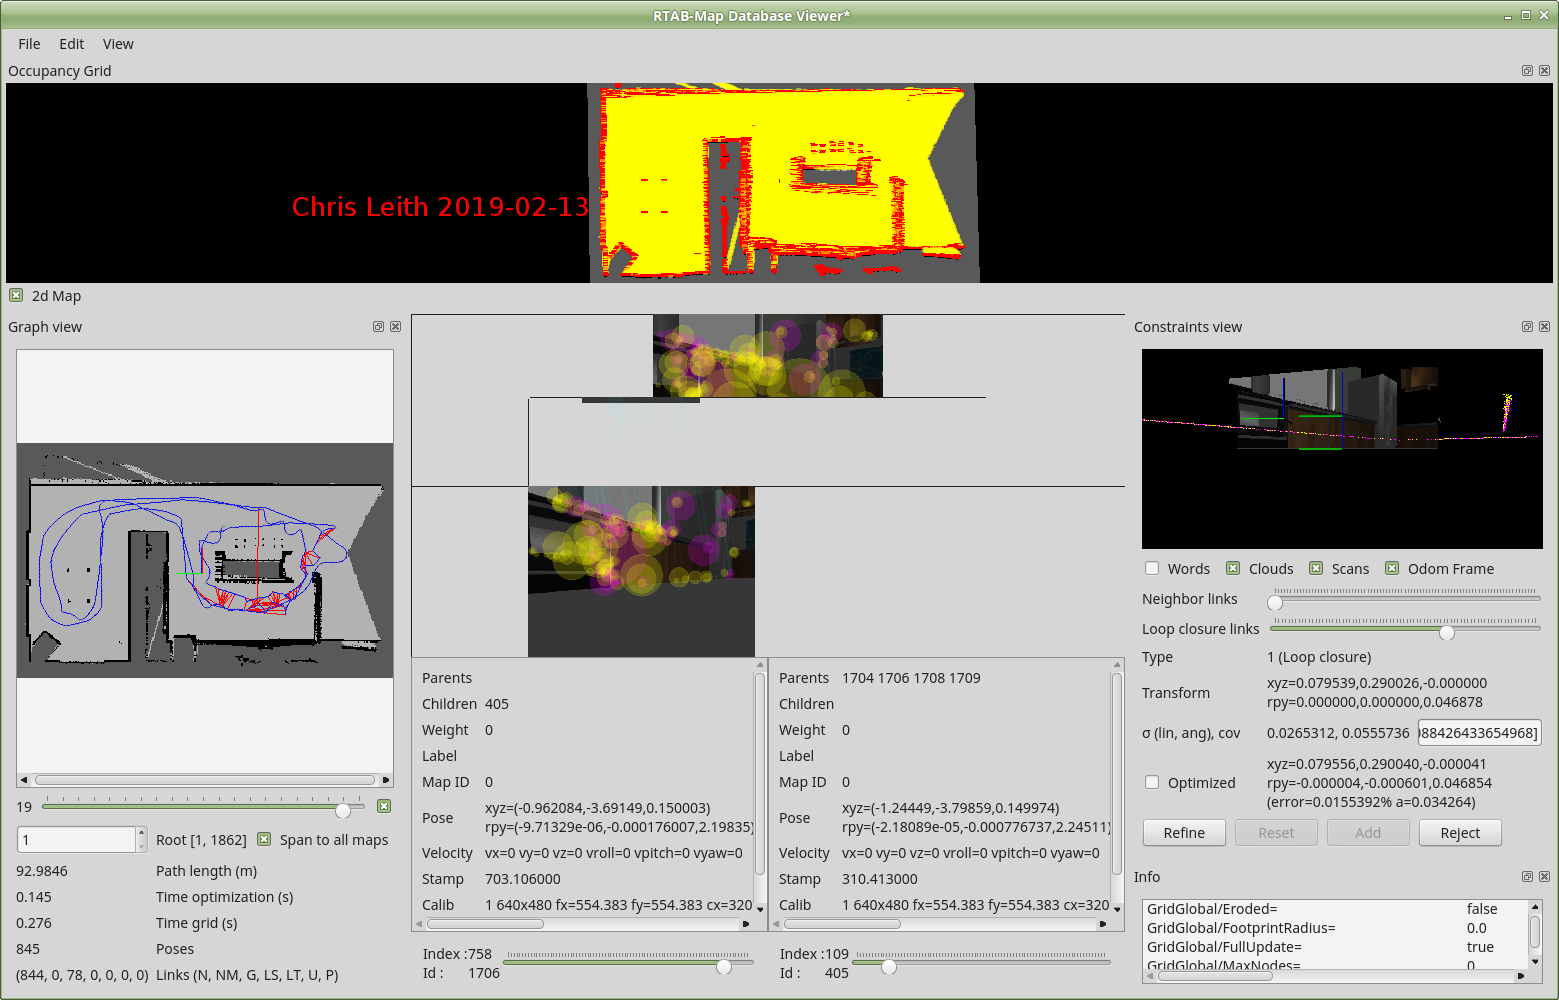
\includegraphics[width=\linewidth]{Assets/DBViewer_kitchen_2019-02-11_19-04-25.png}
      \caption{Kitchen and Dining World DBView Run1}
      \label{fig:kitchen_dbview_run1}
\end{figure}

From Run2 Fig ~\ref{fig:kitchen_dbview_run2} it is seen that RTABMap was able to detect 46 loop closures and generate a recognizable 3D map. However, again some flaws are evident. For example it is evident that RTABMap was unable to detect the correspondence of the stool images and there are thus 'ghost' stool images.

\section{Discussion}
The maps

\section{Conclusion / Future work}
The project 

\end{document}